\section*{Gameplay}
The game is played over a series of six rounds, each of which consists of two or three phases: allocate, vote, and (depending on the outcome of the vote) mutiny.

\subsection*{Allocate}
The captain draws seven random treasure cards face up and proposes an allocation of those treasure cards.

The captain must assign a (possible empty) share of the treasure to each player including themself. Every treasure card must be included in exactly one share.

All players are encouraged to attempt to influence the captain while they try do decide on their proposed allocation.
Ultimately, however, the captain can propose any allocation they like. 

\begin{center}
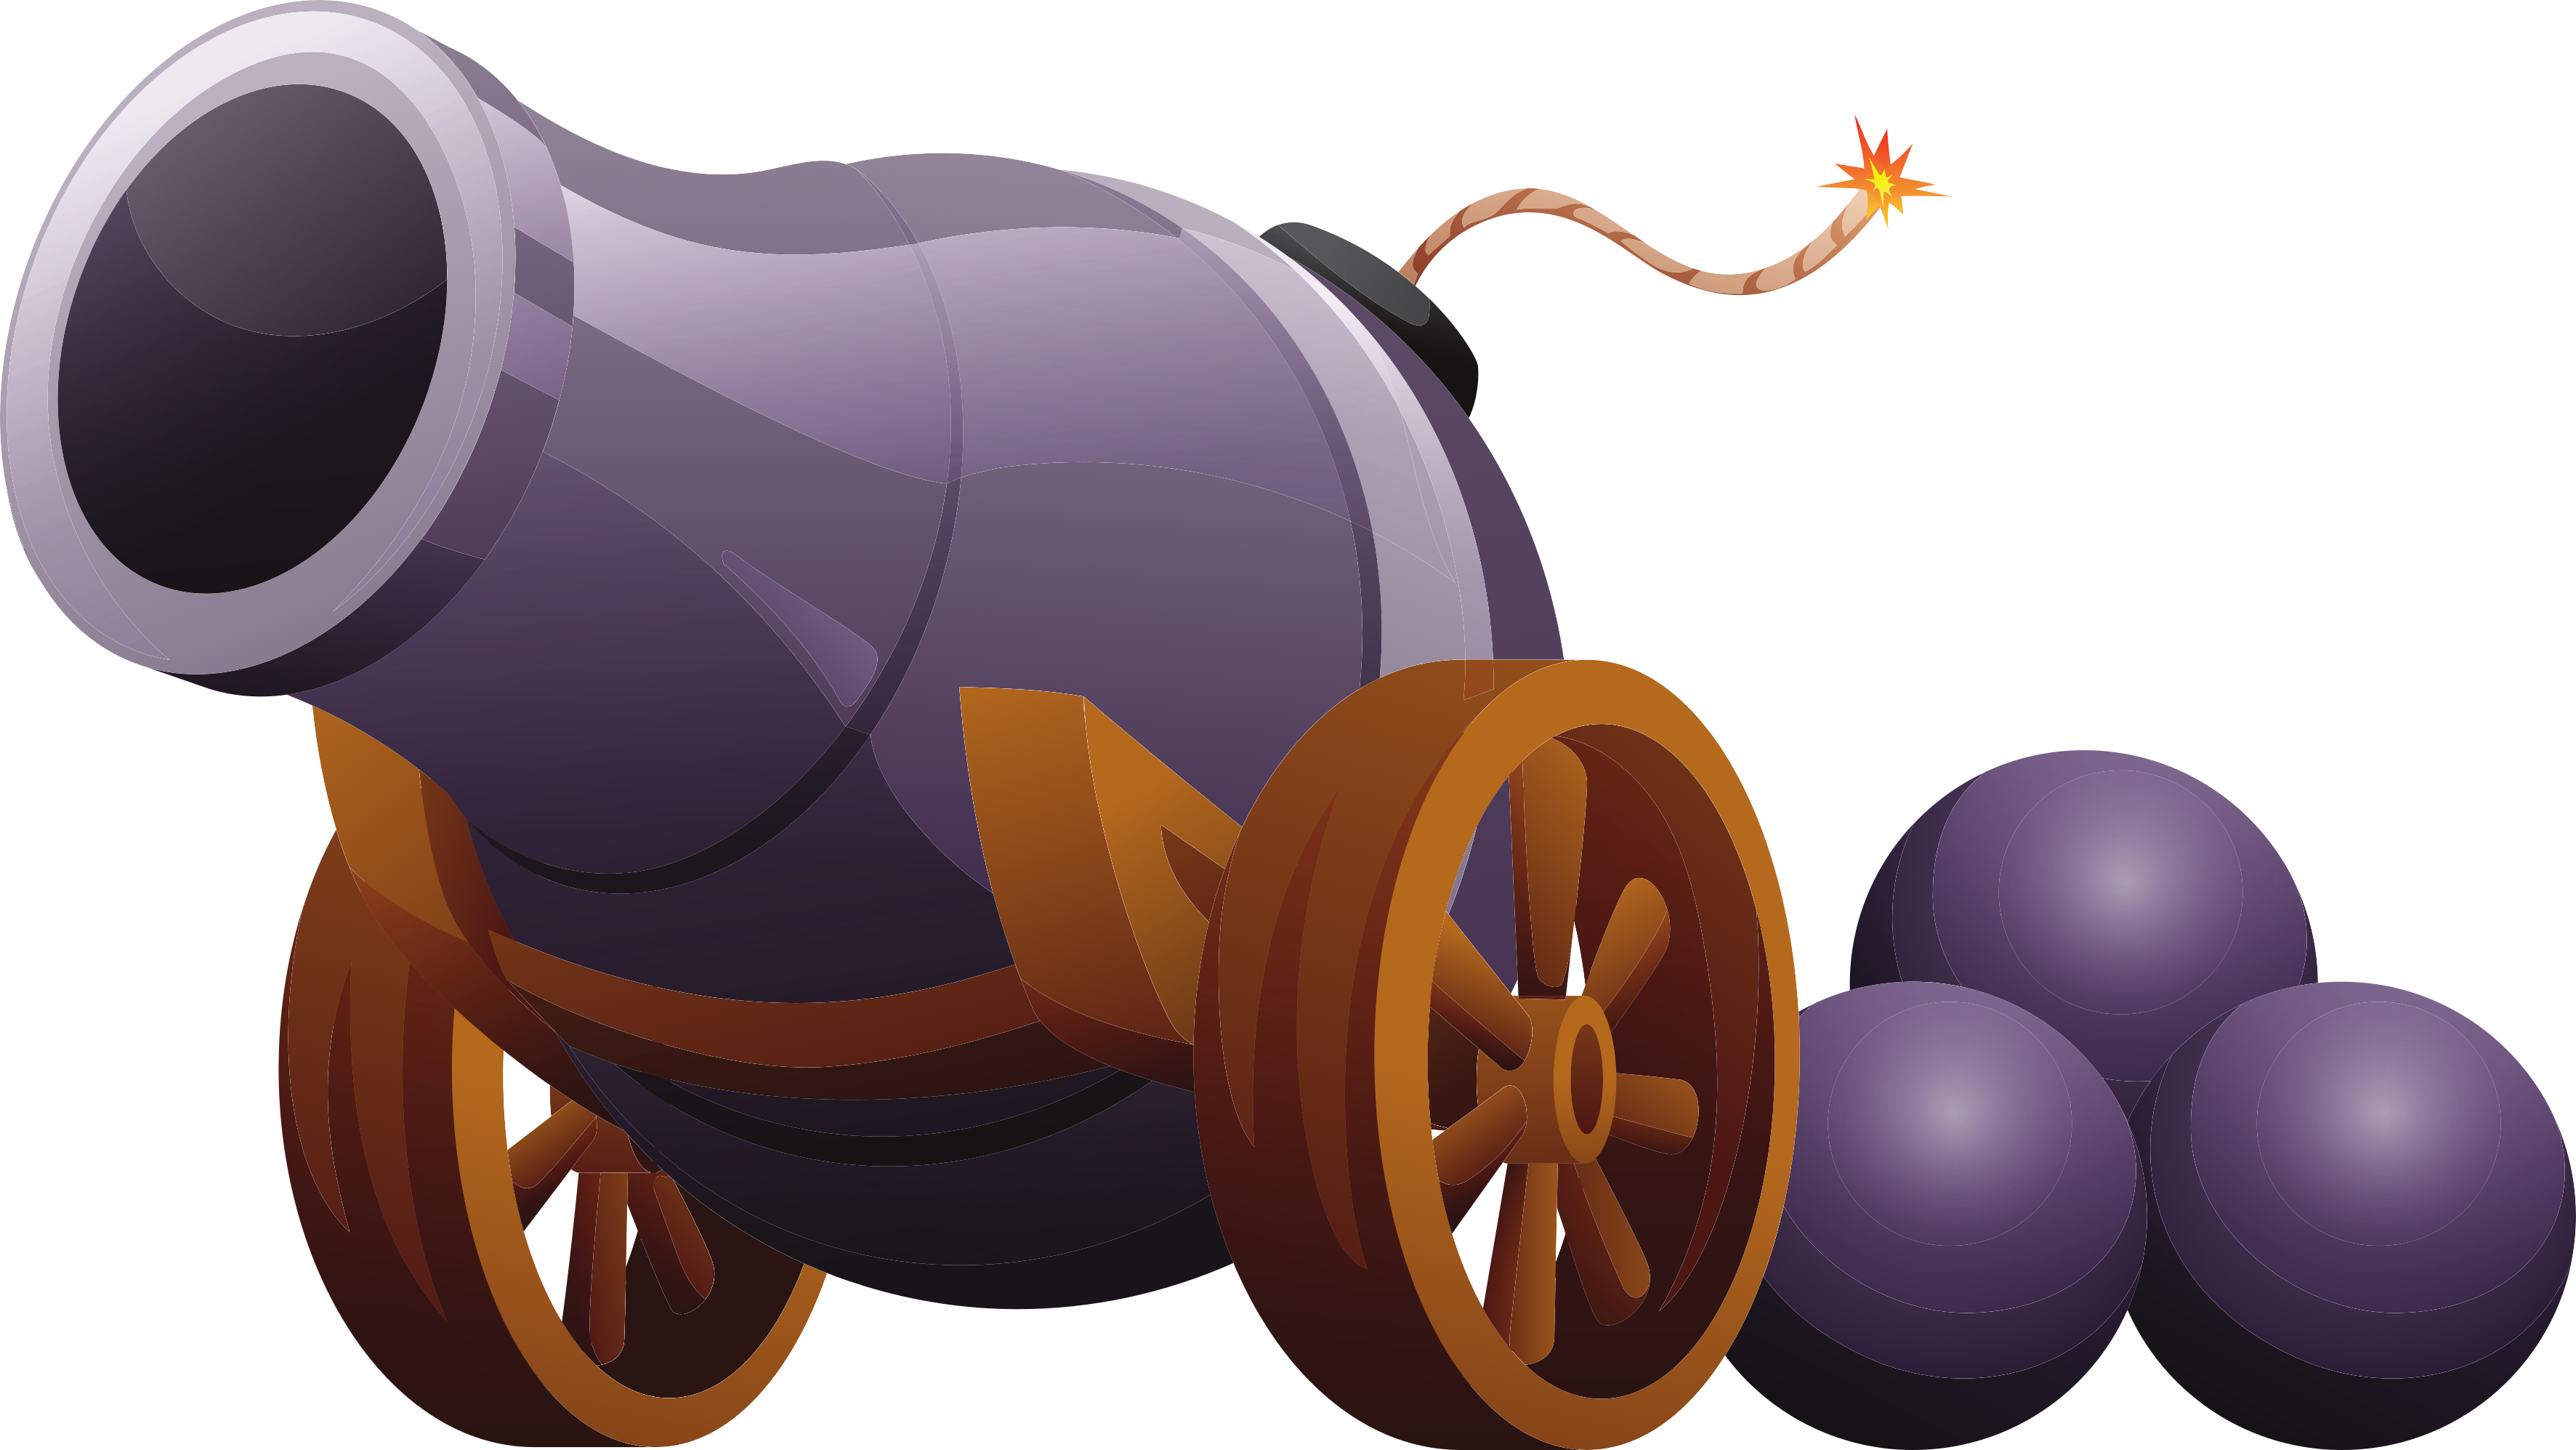
\includegraphics[height=2cm]{Images/cannon.png} \quad \reflectbox{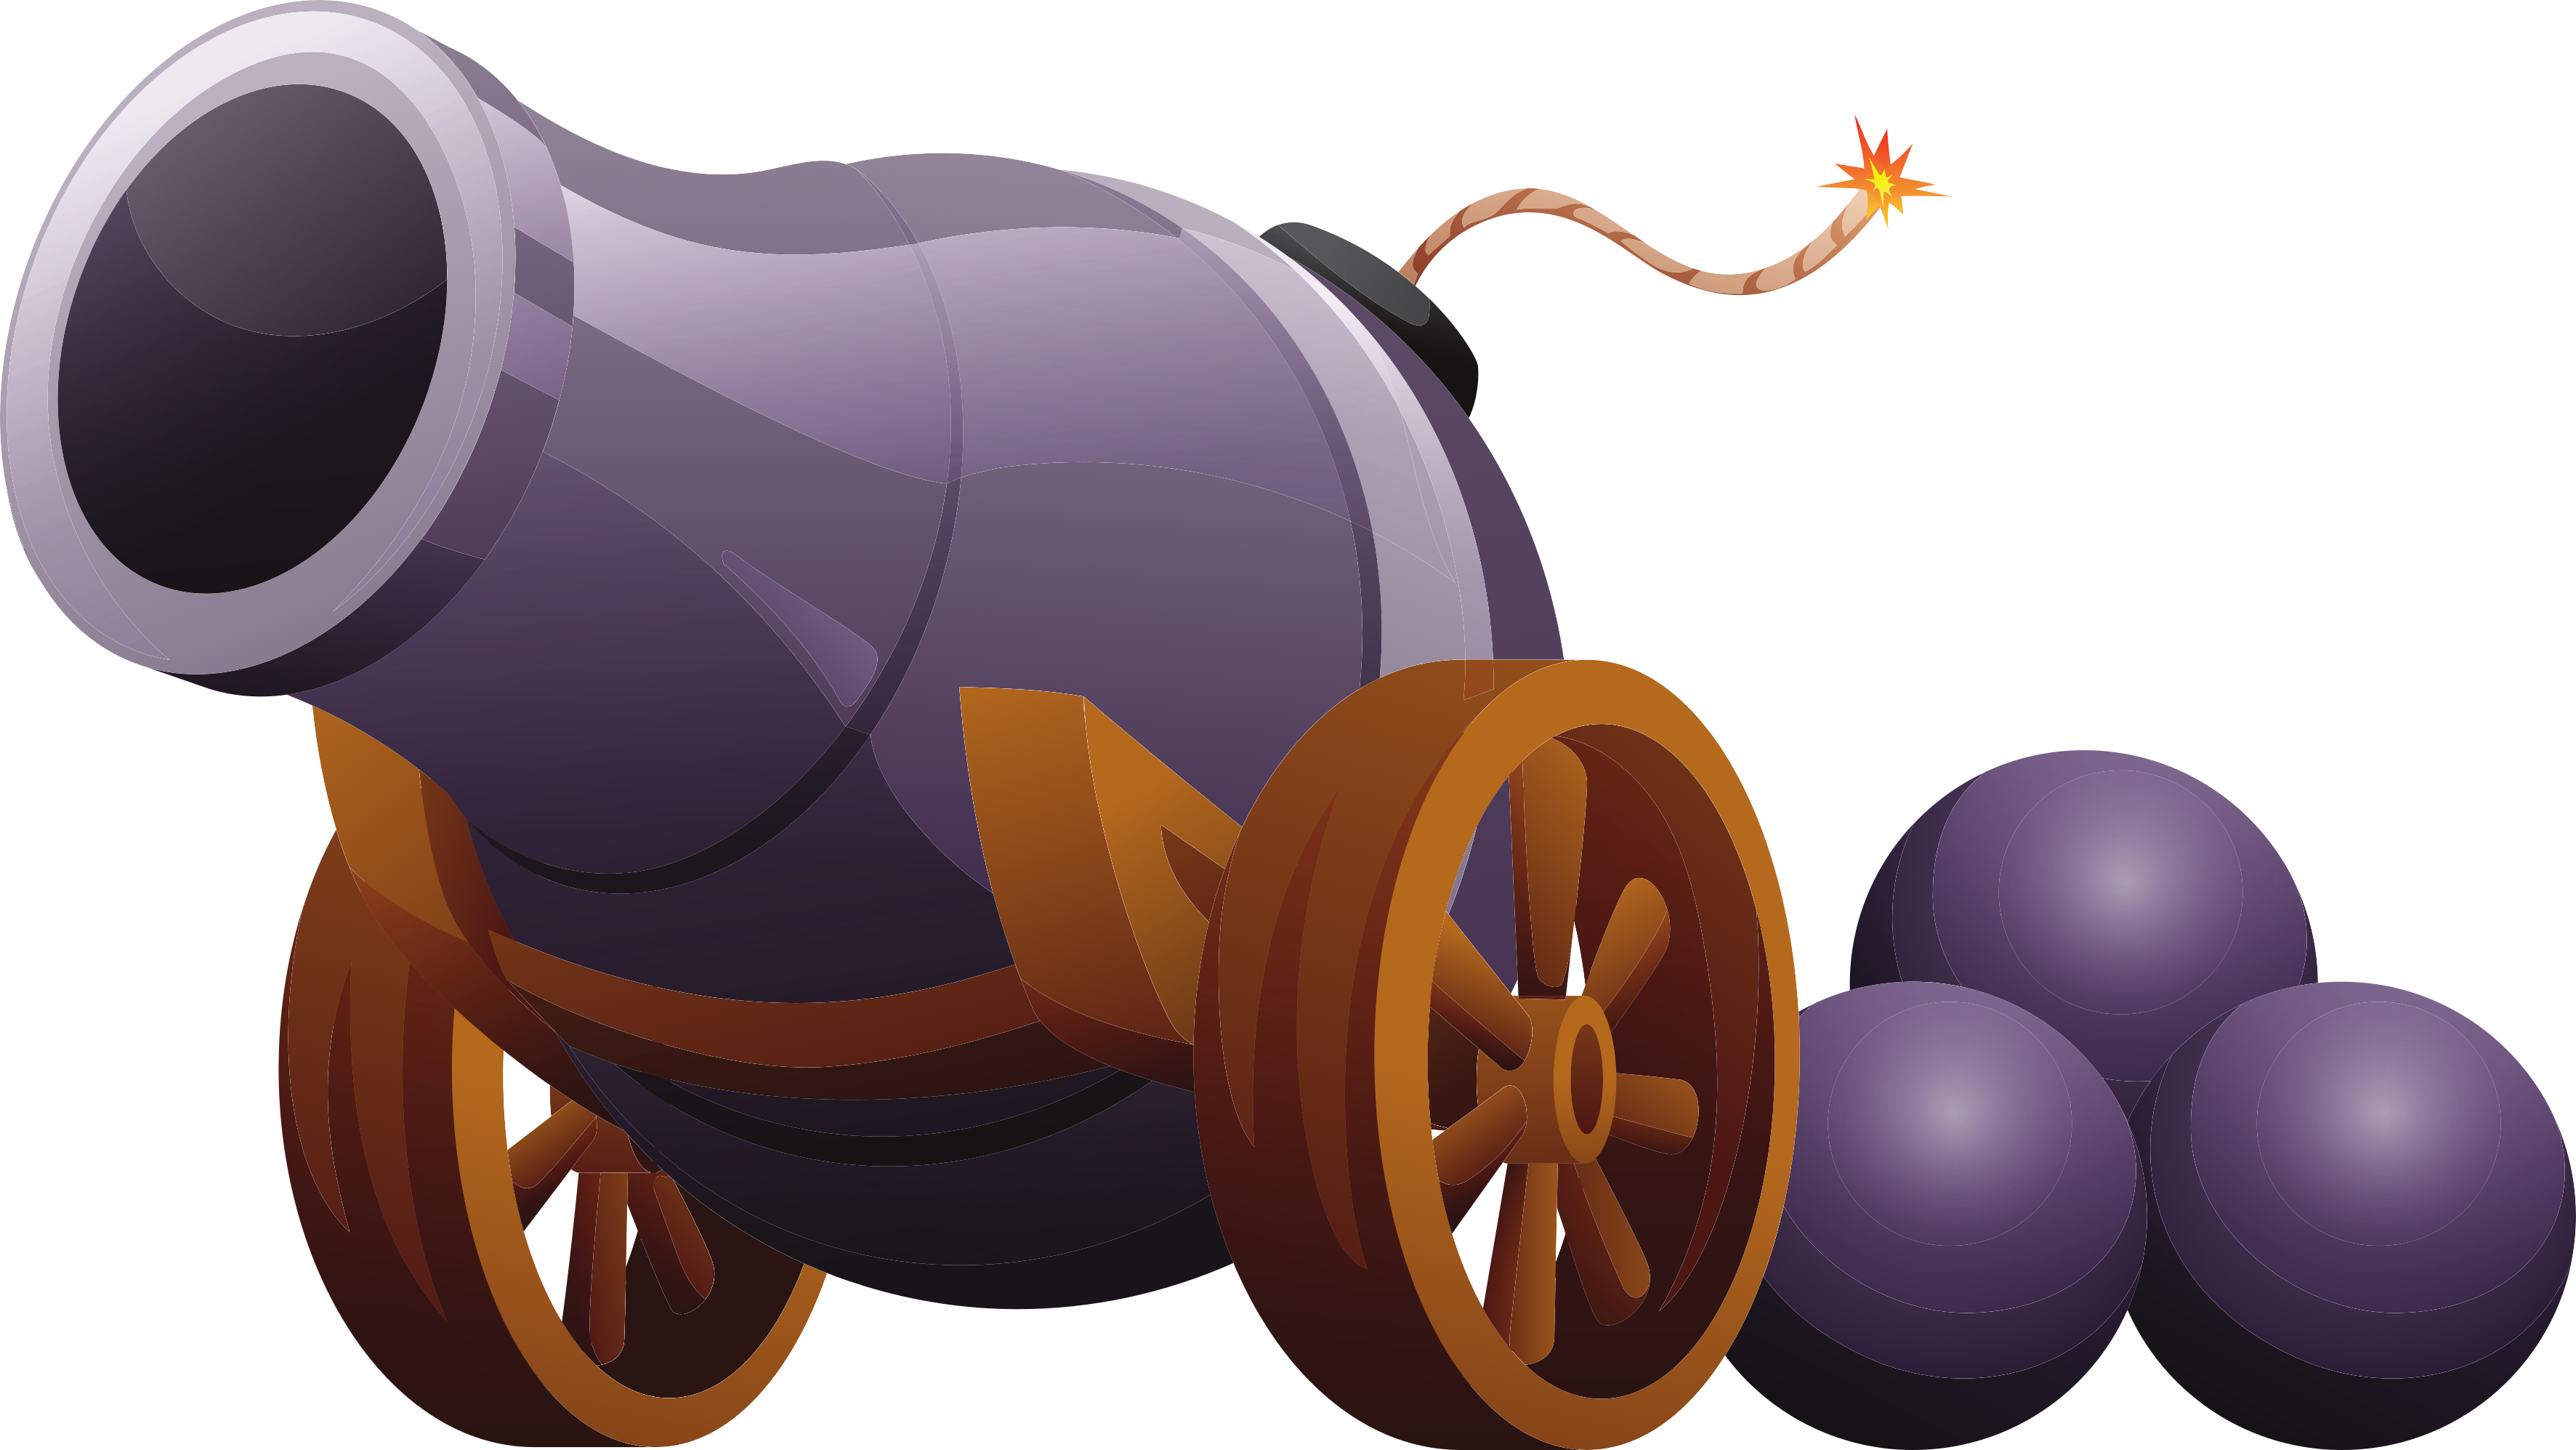
\includegraphics[height=2cm]{Images/cannon.png}}%
\includegraphics[height=1.75cm]{Images/barrel.png} 
\includegraphics[height=1.75cm]{Images/barrel.png}
\end{center}

\newpage

\subsection*{Vote}
All players simultaneously vote on whether to accept the captain's proposed allocation or to reject it.

Each player must either vote \textit{Aye} to accept the captain's proposed allocation or \textit{Nay} to reject it.
Before the game, agree on how you will indicate your votes. A common choice is to use a ``thumbs up'' gesture to indicate \textit{Aye} and a ``thumbs down'' gesture to indicate \textit{Nay}.

\textbf{Note:} The captain must always vote to accept their own proposed allocation.

If a majority of the players voted \textit{Aye}:
\begin{itemize}[leftmargin=*]
\item Players who voted \textit{Aye} keep their allocated shares.
\item Players who voted \textit{Nay} get nothing. Nothing!\\They must discard their allocated shares.
\item The captain retains their position and will serve as captain again for the next round.
\end{itemize}

Otherwise, including the case of a tied vote, the players who voted \textit{Nay} mutiny (see below).

\newpage

\subsection*{Mutiny}
During a mutiny, all players who voted \textit{Nay} during the voting phase this round become mutineers and seize control from the captain.
When they do, they must:
\begin{itemize}[leftmargin=*]
\item Propose an allocation for this round's treasure cards.
\item Choose a mutineer to become the new captain.
\end{itemize}

If the mutineers \textbf{unanimously} agree on both their proposed allocation and their nominee to become the new captain, the mutiny succeeds.
In that case:
\begin{itemize}[leftmargin=*]
\item All players keep their allocated shares.
\item The nominated mutineer becomes the new captain. Give the captain card to the new captain.
\end{itemize}

Otherwise, the mutiny does not succeed. In that case:
\begin{itemize}[leftmargin=*]
\item All of this round's treasures are discarded.
\item The previous captain retains their role.
\end{itemize}

\textbf{Note:} The mutineers can allocate shares to players who are not mutineers. If the mutiny succeeds, all players must keep the shares allocated to them by the mutineers.
